%!TEX root=../robocert.tex
\begin{figure}[htb]
	\centering
	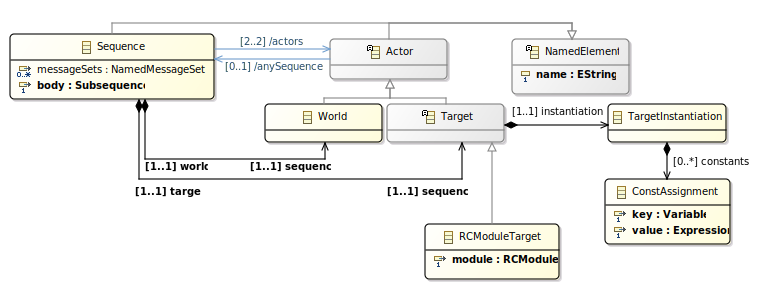
\includegraphics[width=\textwidth]{diagrams/Actors}
	\caption{Class diagram for the part of the \langname{} metamodel dealing with actors.}
	\label{fig:metamodel-actors}
\end{figure}

\noindent
Actors (\mactor{}) capture communication participants in a sequence.
Per \cref{sec:metamodel-sequences}, there are always two actors
attached to a sequence: a \mtarget{} (\cref{ssec:metamodel-actors-target})
and a \mworld{} (\cref{ssec:metamodel-actors-world}).

\Cref{fig:metamodel-actors} depicts the part of the metamodel concerning
actors.

\subsection{\mtarget}\label{ssec:metamodel-actors-target}

A \mtarget{} references the part of a robotic system that serves as the focus
for a particular sequence diagram.  There is
presently one type of target, with more to appear later:

\begin{itemize}
\item
	a \mrcmoduletarget{} references a \mrcmodule.
\end{itemize}

Each \mtarget{} contains a \mtargetinstantiation{} (see below), which
is always applied to any use of that target; assertions may further instantiate
any constants left open by the target's \mtargetinstantiation.

\begin{lstlisting}[style=Example]
module AModule
// RCModuleTarget with implicit empty TargetInstantiation

module AModule
    with { SOME_CONSTANT set to 4, ANOTHER_CONSTANT set to 5 }
// RCModuleTarget with explicit TargetInstantiation
\end{lstlisting}

\subsection{\mtargetinstantiation}

A \mtargetinstantiation{} instantiates some or all of the constants in the
target's parametrisation.  It contains a list of key/value pairs where each key
is a RoboChart \mvariable{} corresponding to a constant, and each value is a
RoboChart \mexpression{} (evaluated in an empty~\todo{check this} scope).

\begin{lstlisting}[style=Example]
{ SOME_CONSTANT set to 4, ANOTHER_CONSTANT set to 5 }
\end{lstlisting}

\subsection{\mworld}\label{ssec:metamodel-actors-world}

A \mworld{} is an \mactor{} that represents the `world' outside a sequence's
\mtarget.  \mworld s contain no data.

\begin{lstlisting}[style=Example]
world
\end{lstlisting}

%%% Local Variables:
%%% mode: latex
%%% TeX-master: "../../robocert"
%%% End:
